\documentclass[conference]{IEEEtran}
\IEEEoverridecommandlockouts
\usepackage{cite}
\usepackage{amsmath,amssymb,amsfonts}
\usepackage{algorithmic}
\usepackage{graphicx}
\usepackage{textcomp}
\usepackage{xcolor}
\usepackage{hyperref}
\usepackage{url}
\usepackage{subfigure}
\def\UrlBreaks{\do\A\do\B\do\C\do\D\do\E\do\F\do\G\do\H\do\I\do\J
\do\K\do\L\do\M\do\N\do\O\do\P\do\Q\do\R\do\S\do\T\do\U\do\V
\do\W\do\X\do\Y\do\Z\do\[\do\\\do\]\do\^\do\_\do\`\do\a\do\b
\do\c\do\d\do\e\do\f\do\g\do\h\do\i\do\j\do\k\do\l\do\m\do\n
\do\o\do\p\do\q\do\r\do\s\do\t\do\u\do\v\do\w\do\x\do\y\do\z
\do\.\do\@\do\\\do\/\do\!\do\_\do\|\do\;\do\>\do\]\do\)\do\,
\do\?\do\'\do+\do\=\do\#} 
\def\BibTeX{{\rm B\kern-.05em{\sc i\kern-.025em b}\kern-.08em
    T\kern-.1667em\lower.7ex\hbox{E}\kern-.125emX}}
\begin{document}

\title{High-Performance scRNA-seq Data Processing with Low-Redundancy Disk Access}

\author{\IEEEauthorblockN{Yu Liu}
\IEEEauthorblockA{\textit{School of Informatics} \\
\textit{Xiamen University}\\
Xiamen, China \\
liuyu123@stu.xmu.edu.cn}
\and
\IEEEauthorblockN{Mingxuan Gao}
\IEEEauthorblockA{\textit{School of Informatics} \\
\textit{Xiamen University}\\
Xiamen, China \\
mingxuangao@stu.xmu.edu.cn}
\and
\IEEEauthorblockN{Lixuan Tan}
\IEEEauthorblockA{\textit{School of Informatics} \\
\textit{Xiamen University}\\
Xiamen, China \\
tanlix@stu.xmu.edu.cn}
\and
\IEEEauthorblockN{Hongjin Liu}
\IEEEauthorblockA{\textit{School of Informatics} \\
\textit{Xiamen University}\\
Xiamen, China \\
liuhongjin@stu.xmu.edu.cn}
\and
\IEEEauthorblockN{Yating Lin}
\IEEEauthorblockA{\textit{School of Informatics} \\
\textit{Xiamen University}\\
Xiamen, China \\
linyating@stu.xmu.edu.cn}
\and
\IEEEauthorblockN{Wenxian Yang}
\IEEEauthorblockA{\textit{Aginome Scientific} \\
Xiamen, China \\
wx@aginome.com}
\and
\IEEEauthorblockN{Rongshan Yu*}
\IEEEauthorblockA{\textit{School of Informatics} \\
\textit{Xiamen University}\\
Xiamen, China \\
rsyu@xmu.edu.cn}
}

\maketitle

\begin{abstract}
High-throughput single-cell RNA sequencing (scRNA-seq) data processing pipelines integrate multiple modules to transform raw scRNA-seq data to gene expression matrices, including barcode processing, sequence quality control, genome alignment and transcript quantification.
With the rapid growth in data volume, the speed of scRNA-seq data processing pipeline has become a major bottleneck to large-scale scRNA-seq studies. 
We present scSpark, a cloud computing based scRNA-seq data processing pipeline. 
By leveraging Apache Spark's in-memory computing capability, scSpark significantly improves the processing speed of scRNA-seq data, and achieves 5\-20 times faster than the state-of-the-art processing pipelines under the same CPU core consumption.
In addition, thanks to Spark's inherent scalability in a cloud computing environment, scSpark can further reduce the processing time for a typical scRNA-seq dataset (e.g., 640 million reads) from hours to minutes when multiple computer nodes (e.g., 16) are used.  
Biological evaluation also confirmed that the results generated by scSpark are highly consistent with existing scRNA-seq data processing pipelines.
\end{abstract}

\begin{IEEEkeywords}
scRNA-seq data processing, Apache Spark, cloud computing
\end{IEEEkeywords}

\section{Introduction}
\begin{figure*}
	\centering
	\includegraphics[width=0.98\textwidth]{fig1.pdf}
	\caption{Using JNI and RDD to integrate the STAR aligner in scSpark.} \label{fig1}
\end{figure*}
Single cell is the fundamental unit of a living organism.
Historically, RNA-seq has been widely used to study gene expression patterns in biological samples.
However, the resolution of bulk RNA-seq could only reach the average level of cell populations. 
With the development of single-cell sequencing technologies, scRNA-seq now allows transcript profiling of tens of thousands of cells simultaneously in a single experiment, and has emerged as a powerful tool to identify and characterize cell types in complex and heterogeneous biological samples~\cite{Zhang2019ComparativeAO}.

Generally, a fully-functioned scRNA-seq data processing pipeline typically implements multiple modules including the unique molecular identifier (UMI) barcode~\cite{Smith2017UMItools} processing, sequence quality control (QC)~\cite{schmieder2011quality}, genome alignment~\cite{Dobin2013STAR,Kim2015HISAT} and transcript quantification~\cite{Parekh2018zUMIs} to convert raw scRNA-seq data into a gene expression matrix for further downstream analysis. 
To enable efficient scRNA-seq data processing, various pipelines have been developed, among which the most influential studies probably include CellRanger~\cite{Zheng2017Massively}, UMI-tools~\cite{Smith2017UMItools}, and STARsolo~\cite{Blibaum2019STARsolo}, etc. 
CellRanger is a highly integrated data processing software tool tailored by 10X Genomics for scRNA-seq data analysis.
It is suitable for processing large datasets on high performance workstations~\cite{Gao2020Comparison}. 
UMI-tools is a comprehensive scRNA-seq data processing suite with the directional barcode collapse algorithm integrated that considerably promotes the transcript quantification accuracy.
STARsolo is a recently developed pipeline extended from the genome aligner STAR to adapt to single cell applications, so that users are enabled to align scRNA-seq reads conveniently to reference genomes using STAR without assistance of any extra tools.

In the big biological data era, 
the computational demand originated from the large volume of scRNA-seq data of increasing numbers of single cell studies is becoming tremendous and surpassed the capabilities of these traditional bioinformatics tools. 
The cloud computing environment is a distributed system with extremely scalable computation capabilities, and allows users to run applications and services on a distributed network using a virtualized system. 
Recently, big data frameworks such as Apache Hadoop (\url{https://hadoop.apache.org}) and Apache Spark (\url{https://spark.apache.org}) have been used to speed up the data processing for next generation sequencing (NGS) data. 
SparkBWA~\cite{Abun2016SparkBWA} exploits the capabilities of Spark to boost the performance of a most widely used NGS data aligner, the Burrows-Wheeler Aligner (BWA). 
GPF~\cite{Li2018Highperformance} is a fast in-memory computing framework designed using the Spark framework for implementing NGS data processing pipelines in cloud computing environment. 
Following the success of cloud-based implementations of NGS data processing pipelines, Falco~\cite{Yang2017Falco} concatenates the genome aligner and transcript quantification software tools using Spark for scRNA-seq data preprocessing.
Although Falco improves the performance of scRNA-seq data processing when a distributed computing environment is available, it does not support UMI barcode processing. Hence, it is incompatible with the widely-used high-throughput scRNA-seq protocols such as 10X Genomics, Drop-seq and Microwell-seq. In addition, it does not leverage the in-memory computing capability of Spark to reduce the disk read and write operations of intermediate data processing steps. Therefore, further performance speedup could be expected. 

To meet the growing computational demand of processing large-scale scRNA-seq data, we present scSpark, an in-cloud and in-memory computing scRNA-seq data processing pipeline with high efficiency and scalability. 
More specifically, by implementing and integrating multiple procedures of a standard scRNA-seq data processing pipeline with the aid of in-memory computing schema of Spark, scSpark eliminates the need for laborious disk read/write operations associated with traditional bioinformatics tools. 
As a result, scSpark is able to improve the speed for scRNA-seq data processing by more than 10 folds compared with other state-of-the-art software tools under the same CPU core consumption. In addition, by harnessing the merit of the parallel computing capability of Spark engine, scSpark further enables users to distribute their scRNA-seq data processing workloads to multiple computational nodes, thus dramatically increases their processing throughput of scRNA-seq data for large-scale studies. 
scSpark is freely available at \url{https://github.com/xmuyulab/spark-scRNASeq-Analysis.git}.

\section{Method}
\subsection{Overview}
Apache Spark~\cite{zaharia2010spark} is a high performance, in-memory and distributed computation engine for large-scale data processing. 
In Spark, Resilient Distributed Dataset (RDD)~\cite{Zaharia2012Resilient} is designed as a read-only data container that can be divided into logical partitions across a cluster of computational nodes for parallel computing. 
By using RDDs, Apache Spark allows to cache data in memory, hence reduces time for redundant disk I/O.
In this study, we developed scSpark based on Spark framework to leverage its two major features for ultra-fast scRNA-seq data processing, namely distributed and in-memory computing. 
Moreover, the workflow of scSpark follows closely with that of UMI-tools. Briefly, our scRNA-seq data processing pipeline consists of three major steps, data loading with whitelist control, alignment of extracted reads to a reference genome, and transcript quantification. 

\subsection{Data loading with whitelist control}
scSpark loads scRNA-seq reads from sequencing result files simlilarly to other software tools. To construct RDD that contains reads for subsequent parallel in-memory processing, e.g., alignment, the following procedures are used (Fig.~\ref{fig1}).

For most data yielded from high-throughtput scRNA-seq platforms, two FASTQ~\cite{cock2010sanger} files are generated to save the paired-end sequencing results where the first FASTQ file contains information of cell barcodes and UMIs, and the second one contains transcript sequences.
First, scSpark loads scRNA-seq reads from disks in parallel into two RDDs, which are FASTQ R1 RDD for the first read and FASTQ R2 RDD for the second read respectively by using \textit{newAPIHadoopFile} Spark function and reimplementing Hadoop-BAM~\cite{hadoopBAM}.

Subsequently, scSpark extracts cell barcodes and UMIs from FASTQ R1 RDD as a key-value structure where the key is cell barcode and the value is UMI. Then the highest-occurrent cell barcodes are identified with a user-defined threshold to create the Whitelist RDDs~\cite{guo2018bioinformatics}, so that the unwanted reads can be discarded with \textit{join} function. \textit{zipWithIndex} function is used to index both read-pair FASTQ RDD to preserve the corresponding relationship of the cell barcode, UMI and transcript sequence.

\subsection{Parallel genome alignment}

As in CellRanger, UMI-tools and STARsolo, we also adopt STAR as the aligner in scSpark.
The conventional STAR alignment procedure loads raw reads from FASTQ files and writes alignment results to Sequence Aligment/Map (SAM) or the compressed binary version of a SAM (BAM)~\cite{li2009sequence} file, requiring extensive disk access which consumes a significant amount of time.

Instead, in scSpark, we use the Java Native Interface (JNI)~(\cite{kim2012benchmarking}) to directly feed FASTQ RDD to STAR, and further transfer the results output from STAR to the SAM RDD after alignment (Fig.~\ref{fig1}.a). 
In such way, the alignment process is performed in an in-memory computing manner without any redundant disk access causes from temporyary result. 

To balance the workloads across different nodes for parallel processing, we use the Spark function \textit{repartition} before alignment to split FASTQ RDDs into \textit{N} subsets where \textit{N} denotes the number of nodes available in the cluster.
After data partitioning and shuffling, the STAR alignment is performed in parallel on each computational nodes, directly resulting in a SAM RDD which is used as an input to the next module.

\subsection{Transcript quantification}
For transcript quantification, we first use the \textit{textFile} function in Spark to load the gene transfer format (GTF)~\cite{breese2013ngsutils} file which contains the gene annotation information into memory as GTF RDDs (Fig.~\ref{fig1}.b). 
After alignment, both SAM RDDs and GTF RDDs are respectively grouped by chromosome into Grouped SAM RDDs and Grouped GTF RDDs respectively for parallel processing by the Spark function \textit{groupBy}. 

Then, we combine Grouped GTF RDD and Grouped SAM RDD with the same chromosome to obtain Chromosome Partition RDD by using the \textit{join} function.
At this stage, the gene names are assigned to each read according to its alignment coordinates by a user-defined \textit{flatMap} function. 

Subsequently, we reimplemented the directional algorithm designed by UMI-tools for transcript quantification in parallel. The quantification resutls are saved in Counted RDD.

Finally, the resulting expression matrix are generated on each node and wrote to disk or distributed file system by using default Spark's action function like \textit{saveAsTextfile} for further downstream analysis. 

\section{Results}

\begin{figure*}
	\centering
	\subfigure[Barcode extraction and sequence quality control.]{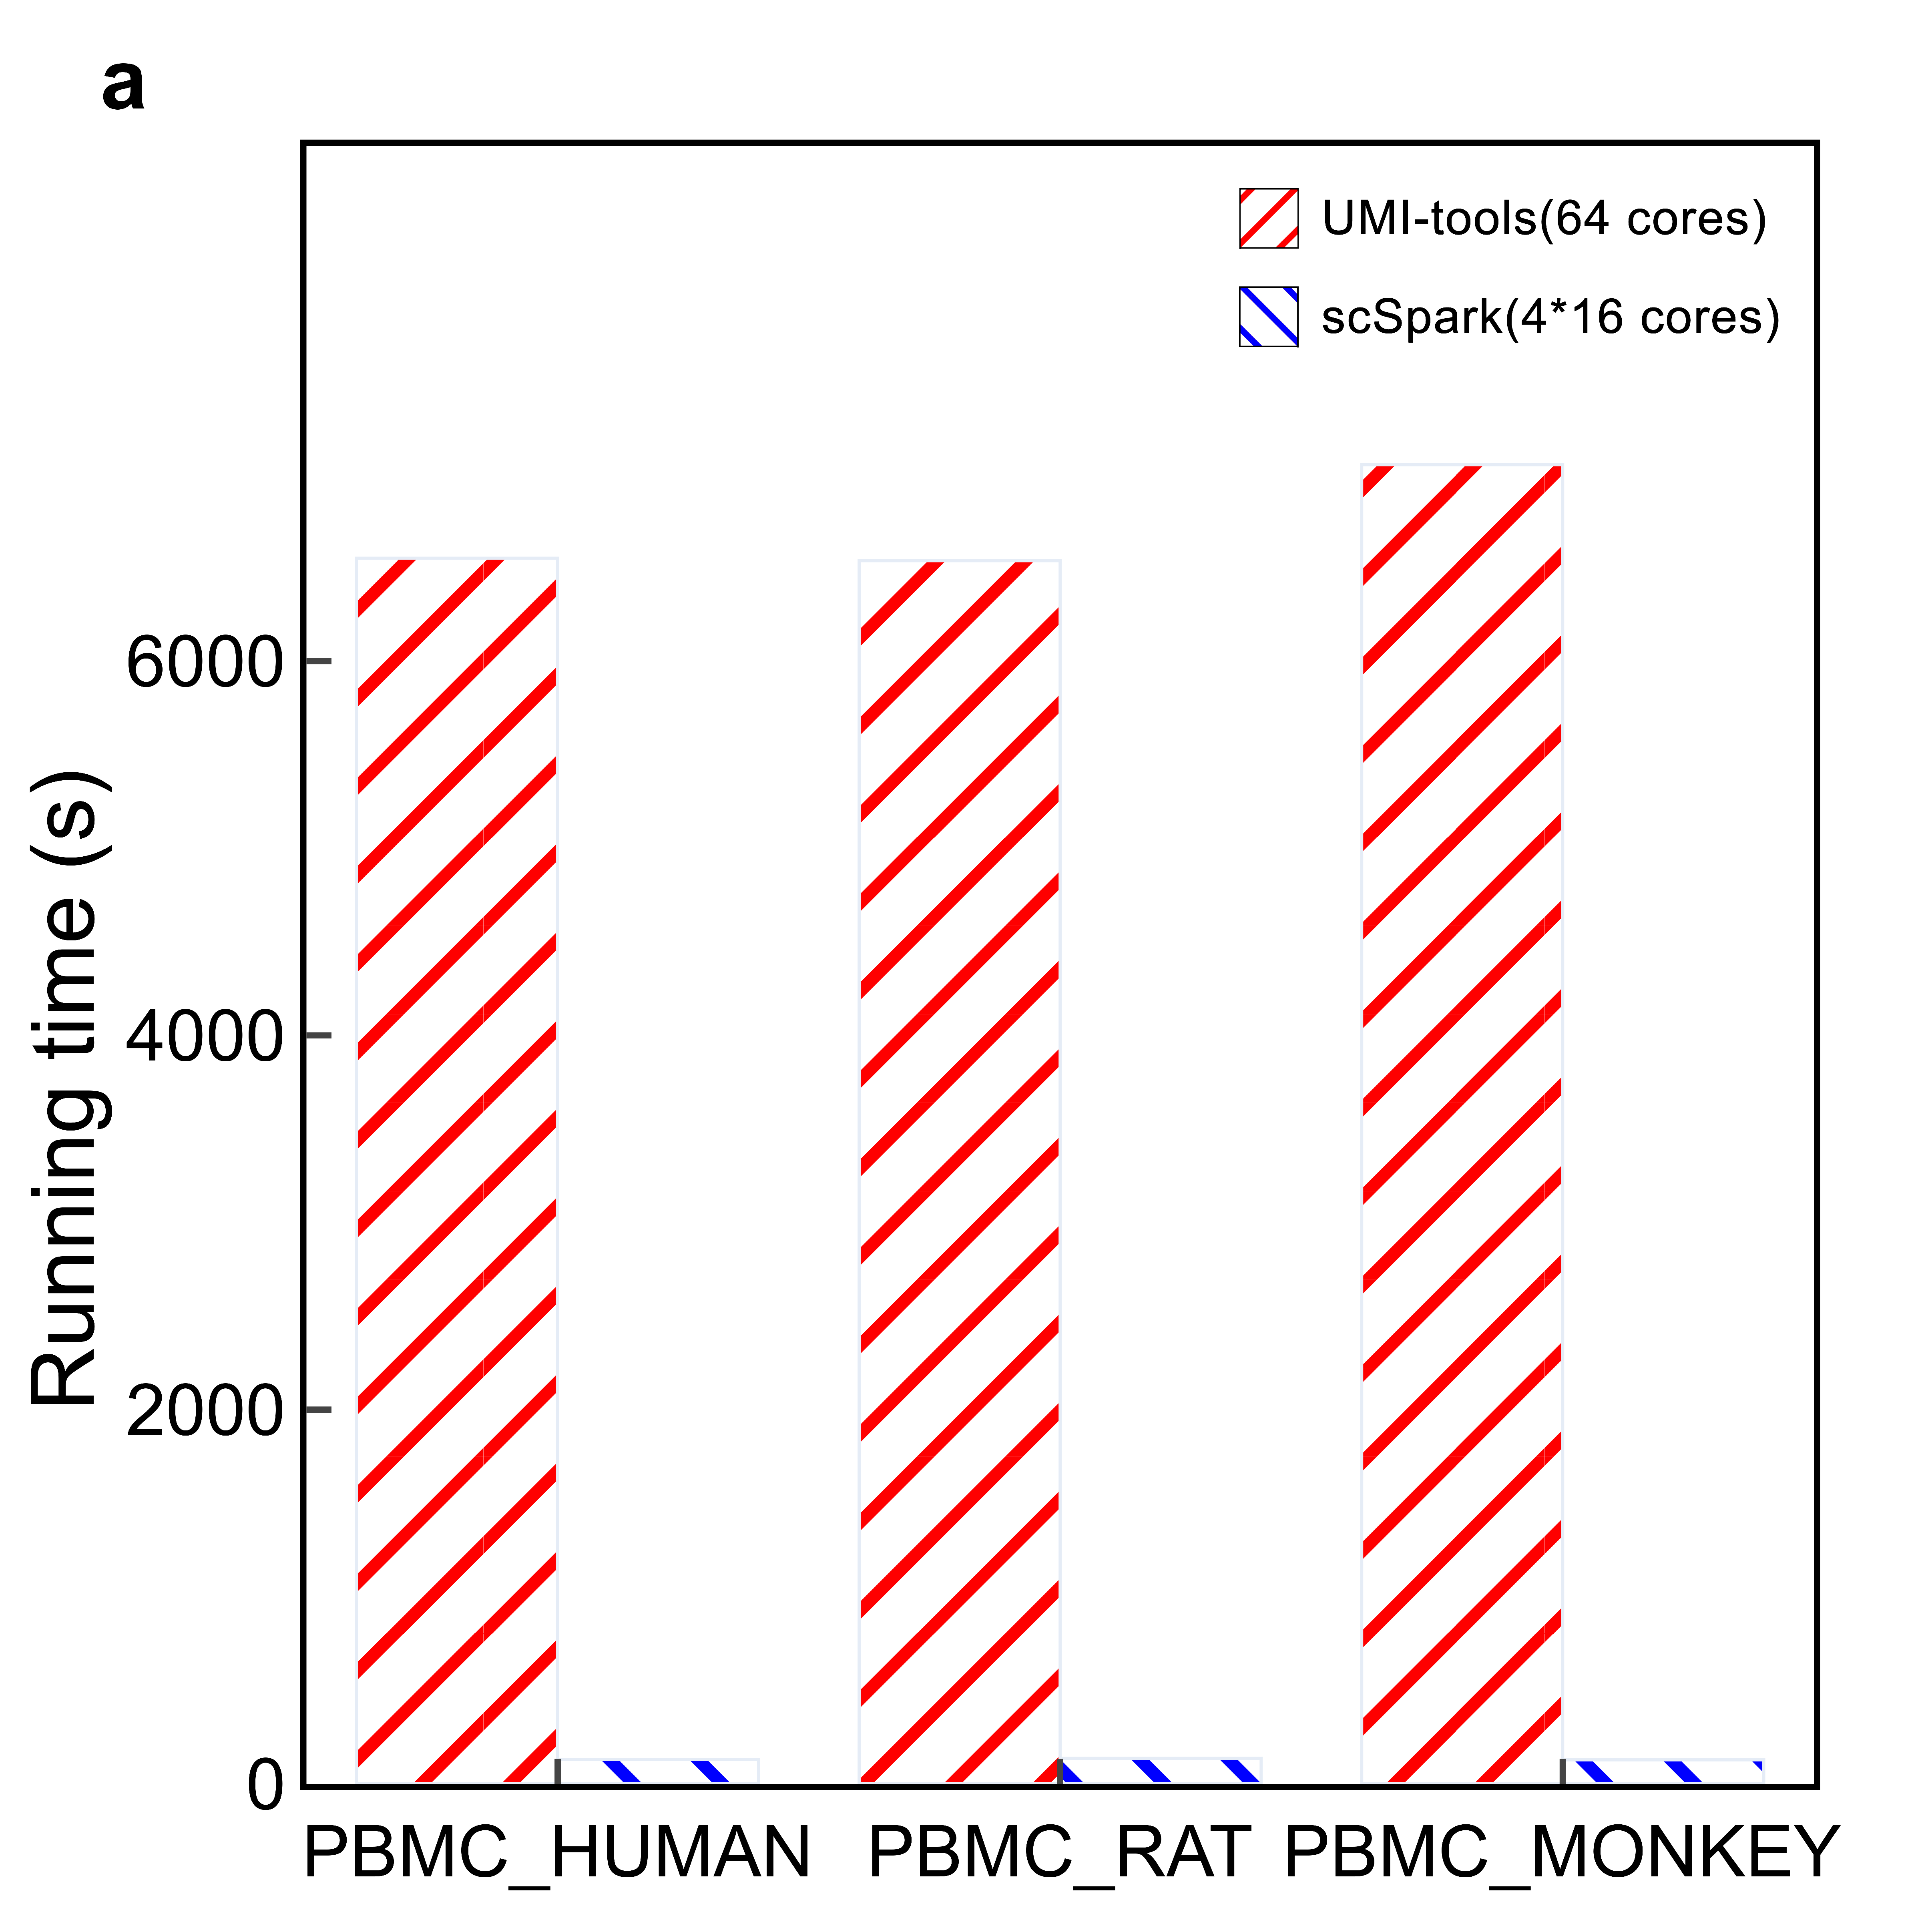
\includegraphics[width=0.32\textwidth]{fig2a.pdf}}
	\subfigure[Alignment.]{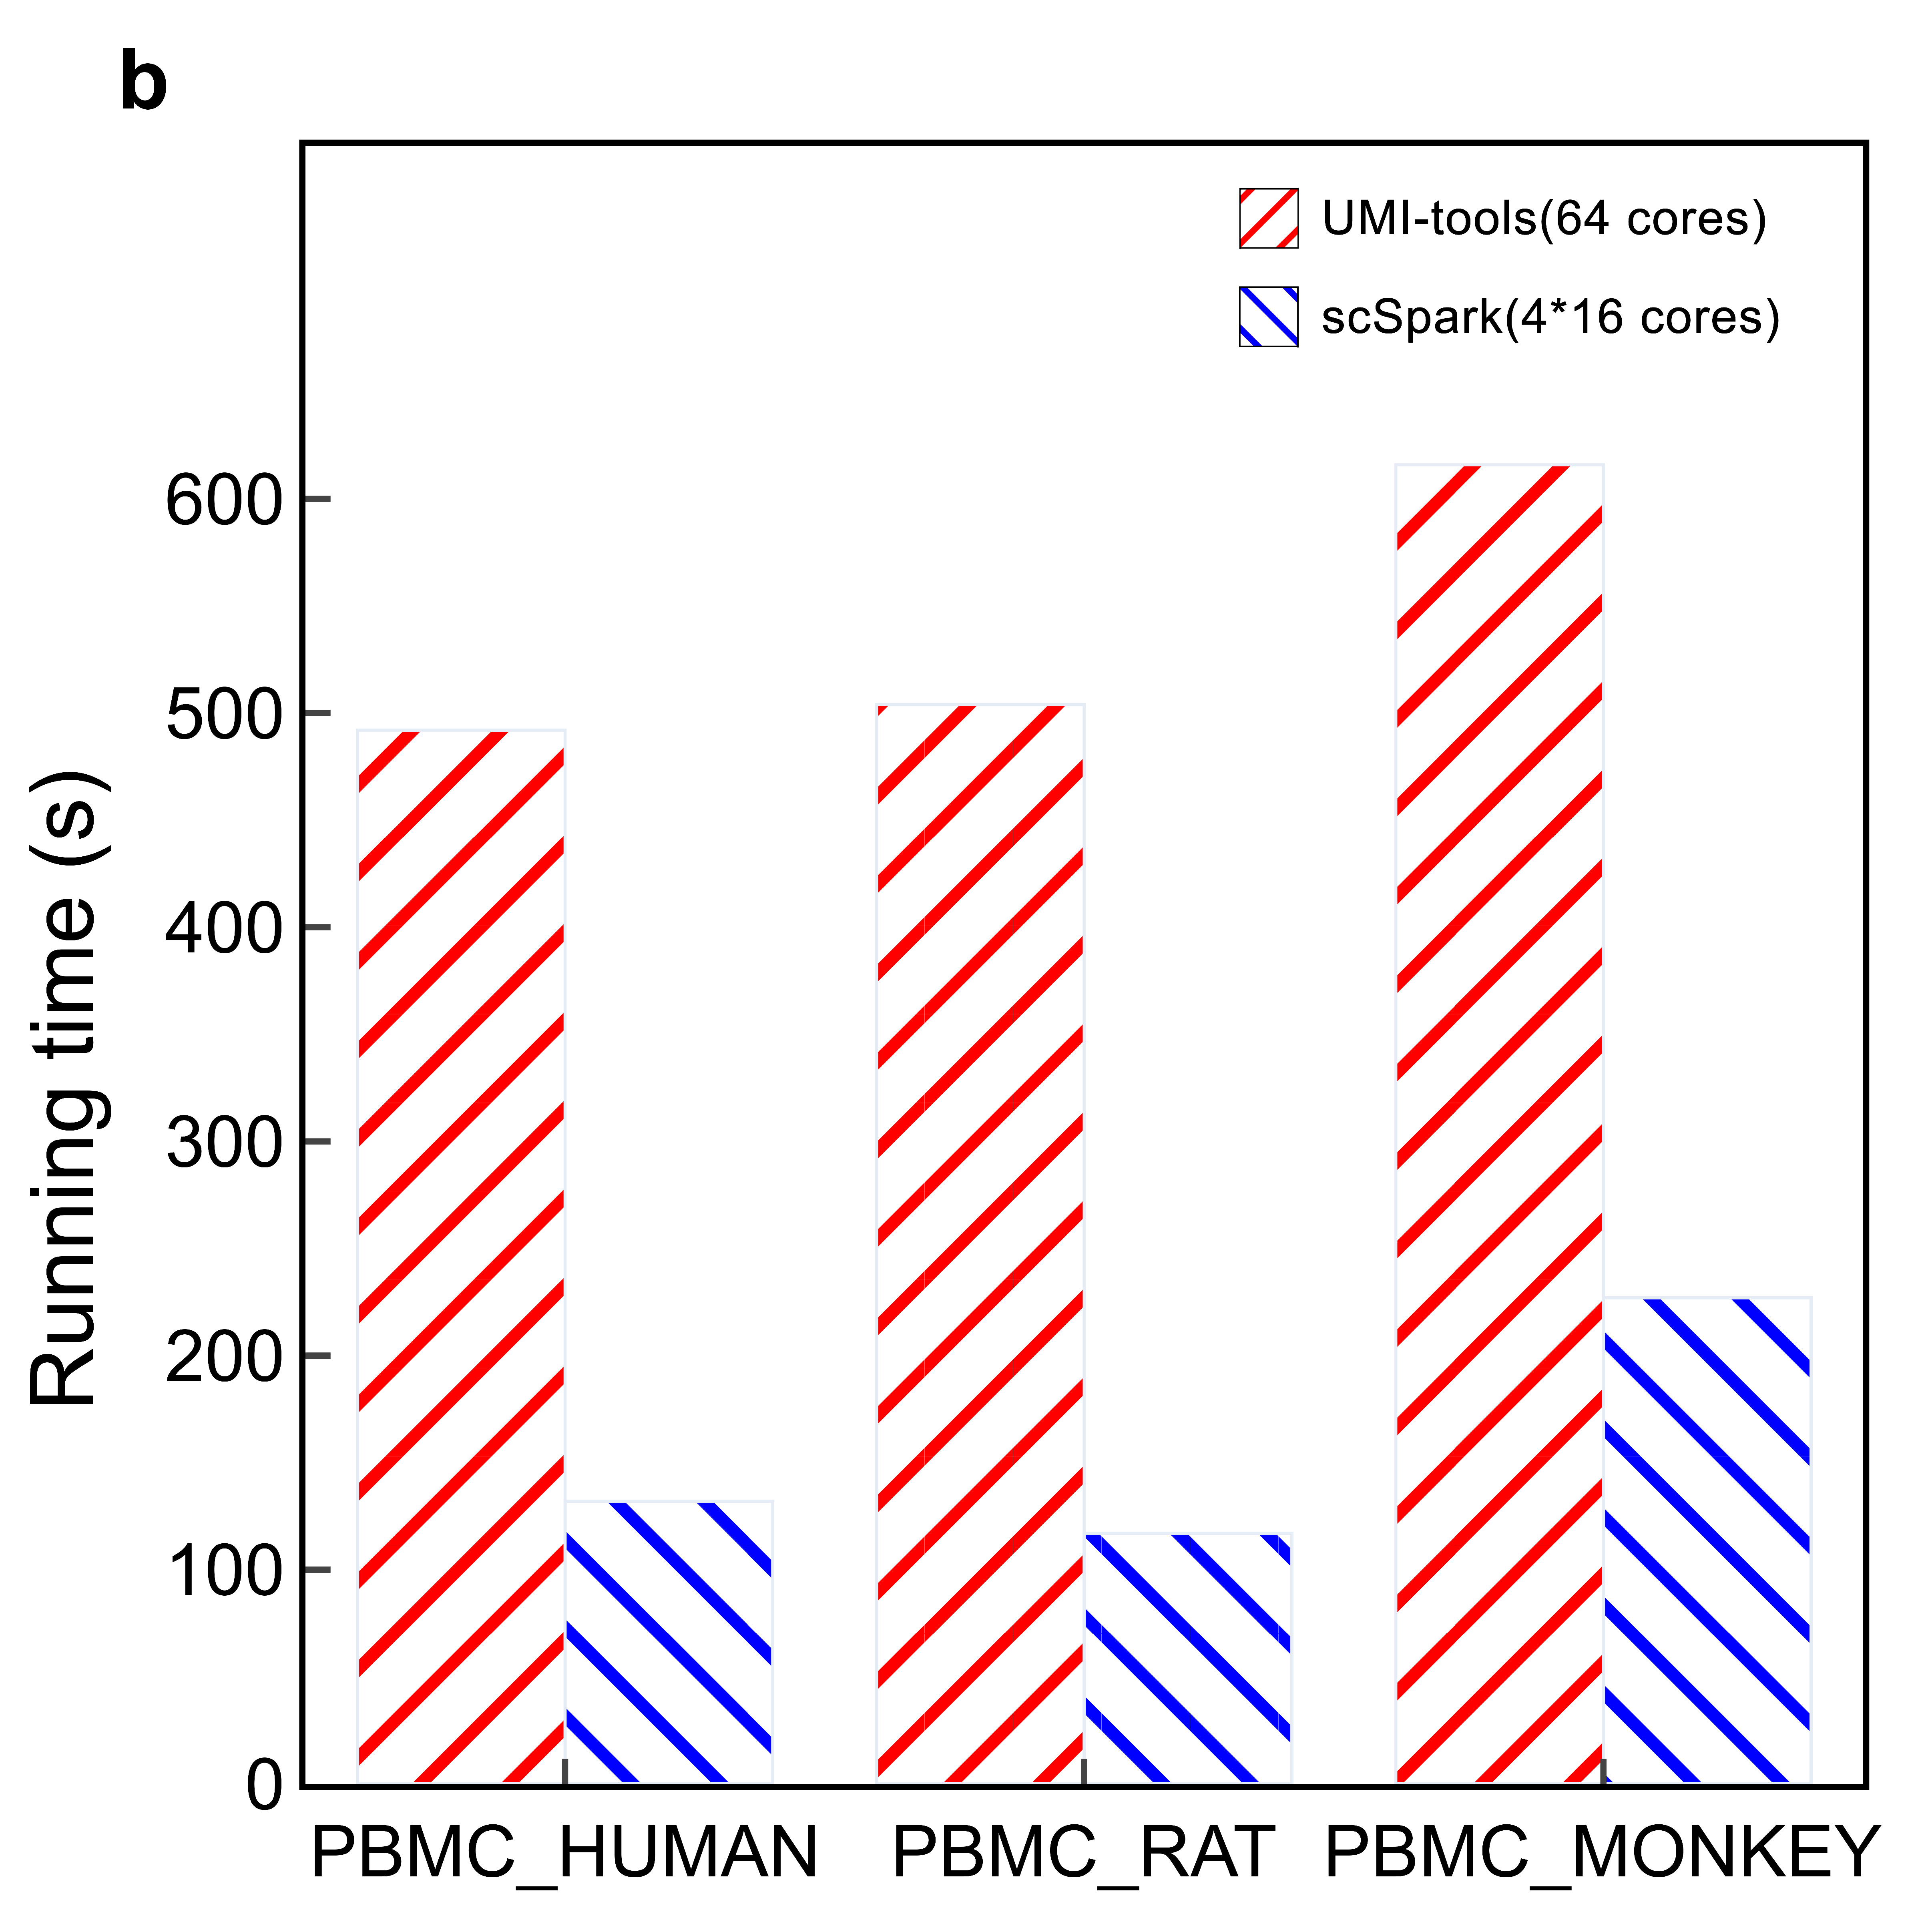
\includegraphics[width=0.32\textwidth]{fig2b.pdf}}
	\subfigure[Transcript counting.]{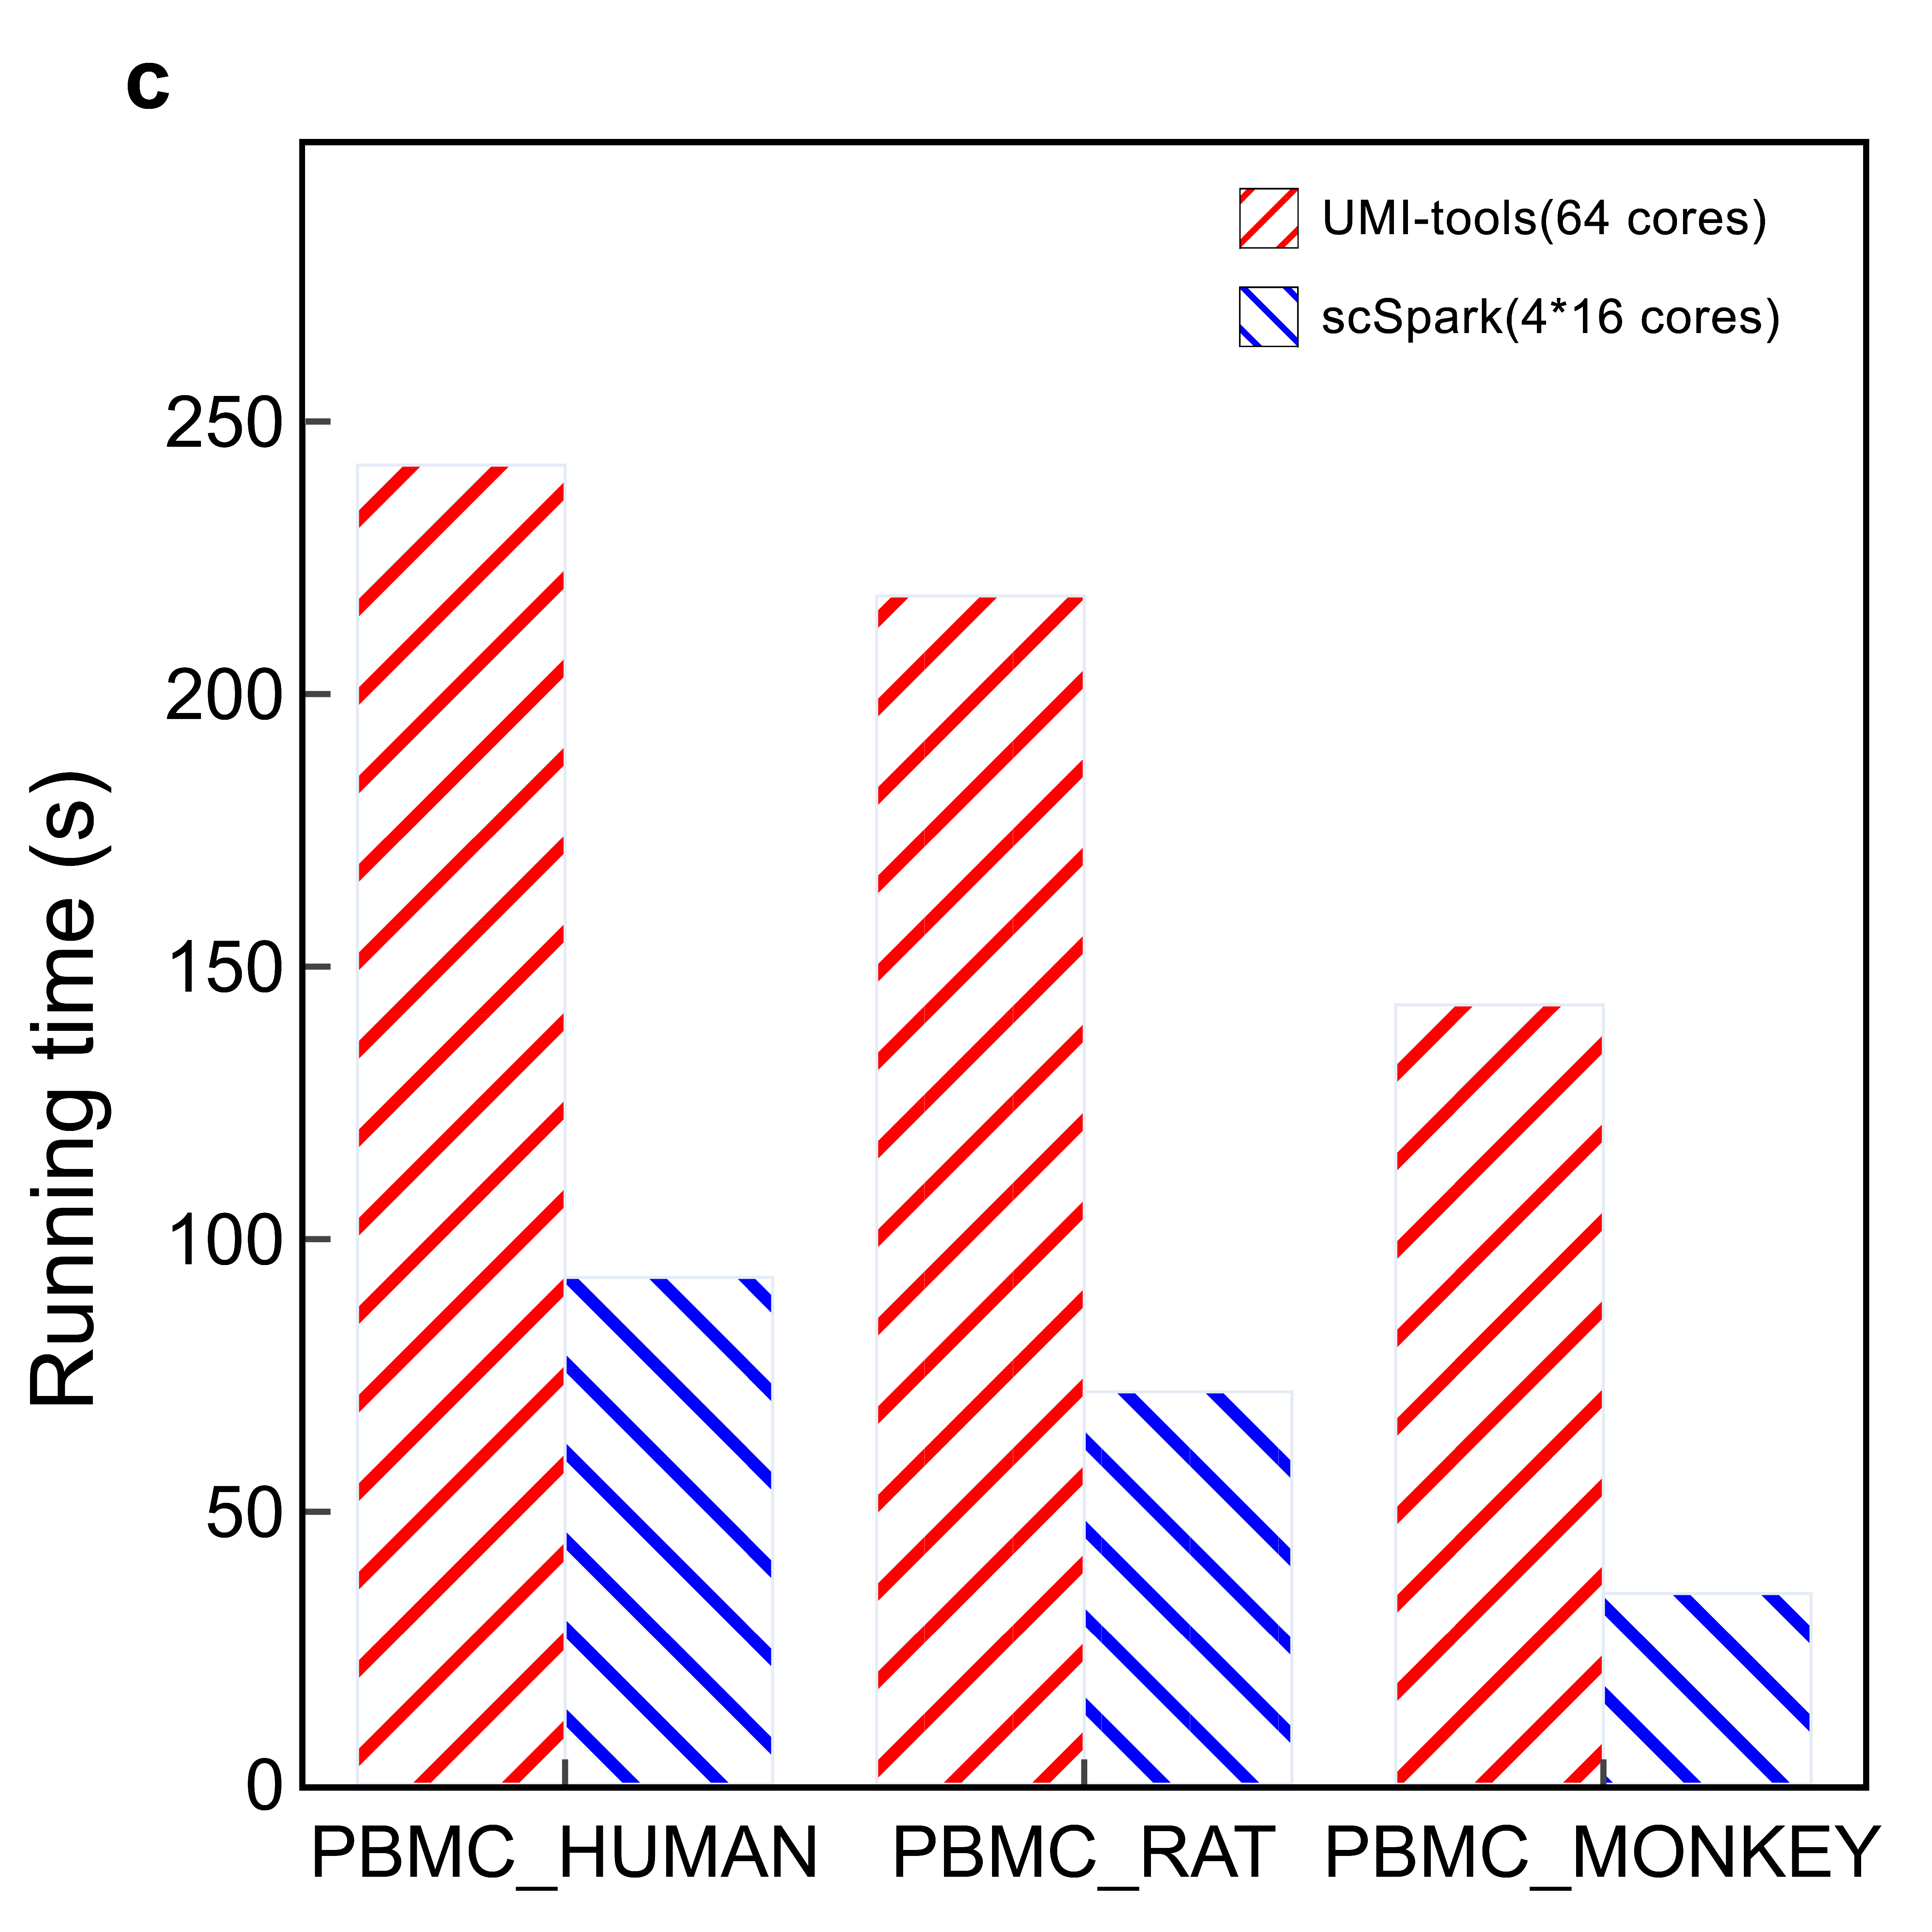
\includegraphics[width=0.32\textwidth]{fig2c.pdf}}
	\caption{Comparison of UMI-tools and scSpark's each step.}
	\label{fig2}
\end{figure*}

\subsection{Experiment design}
The performance in processing speed of scSpark is compared with CellRanger, UMI-tools and STARsolo. 
We used Apache Spark (version 2.1.0) as scSpark's in-memory computing environment.
Our Spark cluster used up to 8 workstations, each workstation is configured with up to 32 \textit{Intel Xeon(Cascade Lake) Platinum 8269CY} CPU cores at 2.5GHz.
And we split each workstation to two Spark's executor logically.
Each Spark's executor contains of 16 CPU cores and 64 GBytes of DRAM.
In traditional pipelines' experiments, we use workstation with 64 \textit{Intel(R) Xeon(R) CPU E5-2683 v4} CPU cores at 2.1GHz.
And this workstation consists of 256 GBytes DRAM.
Pre-tests were performed to ensure sufficient memory for each pipeline.

Three scRNA-seq datasets containing peripheral blood mononuclear cells (PBMCs) from three different species, namely human, rat and monkey, generated by 10X Genomics platform were used in our experiments. 
In total, there are approximately 640 millions, 289 millions and 262 millions reads in the raw data of the PBMC\_human, PBMC\_rat and PBMC\_monkey datasets, respectively. 
In all the experiments, we run all the four pipelines with exactly the same cell number and barcode pattern arguments.

Firstly, we compared scSpark's performance on a cluster with 64 (16$\times$4) CPU cores with the other three pipelines' performance on a workstation on 64 CPU cores on PBMC\_human.
In all experiments, the number of CPU cores used was configured using the \textit{runThreadN} parameter for STAR and STARsolo, the \textit{localcores} parameter for CellRanger and the \textit{SPARK\_EXECUTOR\_CORES} parameter for scSpark. 
To test improvement in each step performance of scSpark, we meatured process time of UMI-tools and scSpark each substep to prove scSpark get improve in any single substep on 64 CPU cores.

Then we tested performance of each pipelines on PBMC\_human when CPU cores number is up to 64.
Due to limit of single workstation CPU cores, we tested STARsolo and CellRanger's speedup from 32 CPU cores to 64 CPU cores.
And due to limit of memory capacity per node, we tested scSpark's speedup in 32 (2$\times$16) CPU cores, 48 (3$\times$16) CPU cores to 64 (4$\times$16) CPU cores.
Moreover we tested performance of scSpark on PBMC\_human when CPU cores number is between 128 and 256.

Particularly, we tested the mapping speed of STAR on PBMC\_human dataset when CPU cores number is up to 64.
Furthermore, we tested the mapping speed of scSpark on three datasets when CPU cores number is between 128 and 256.

Also we splited PBMC\_human dataset into 80 millions, 160 millions and 320 millions reads.
We processed PBMC\_human and three sub datasets on scSpark with different CPU cores number condition.
After that we compare each dataset's performance to evaluated whether FASTQ data volume will influence scSpark's performance.

Our scSpark is developed based on UMI-tools and UMI-tools accuracy was fully verified. 
This section we used the gene expression matrix that was obtained by scSpark and UMI-tools under the same dataset to perform downstream analysis of scRNA-seq data. 
And then we compared two tools transcript analysis's result and cell cluster analysis's result to verify the correlation between scSpark and UMI-tools. 
Under PBMC\_human dataset, we used scSpark and UMI-tools to get gene express matrix, compared two tools' result, and computed their correlation.

\subsection{Efficiency evaluation}

\begin{table}
	\centering
	\caption{Comparison of processing time (seconds) of four pipelines.}\label{tab1}
	\begin{tabular}{l | l | l | l }
		\hline
		 & PBMC\_human & PBMC\_rat & PBMC\_monkey \\ 
		\hline
		UMI-tools & 7284 & 7259 & 7809 \\
		CellRanger & 2225 & 1999 & 1891 \\
		STARsolo & 1987 & 1854 & 2357 \\
		\textbf{scSpark} & \textbf{355} & \textbf{326} & \textbf{391} \\
		\hline
	\end{tabular}
\end{table}

\begin{figure*}
	\centering
	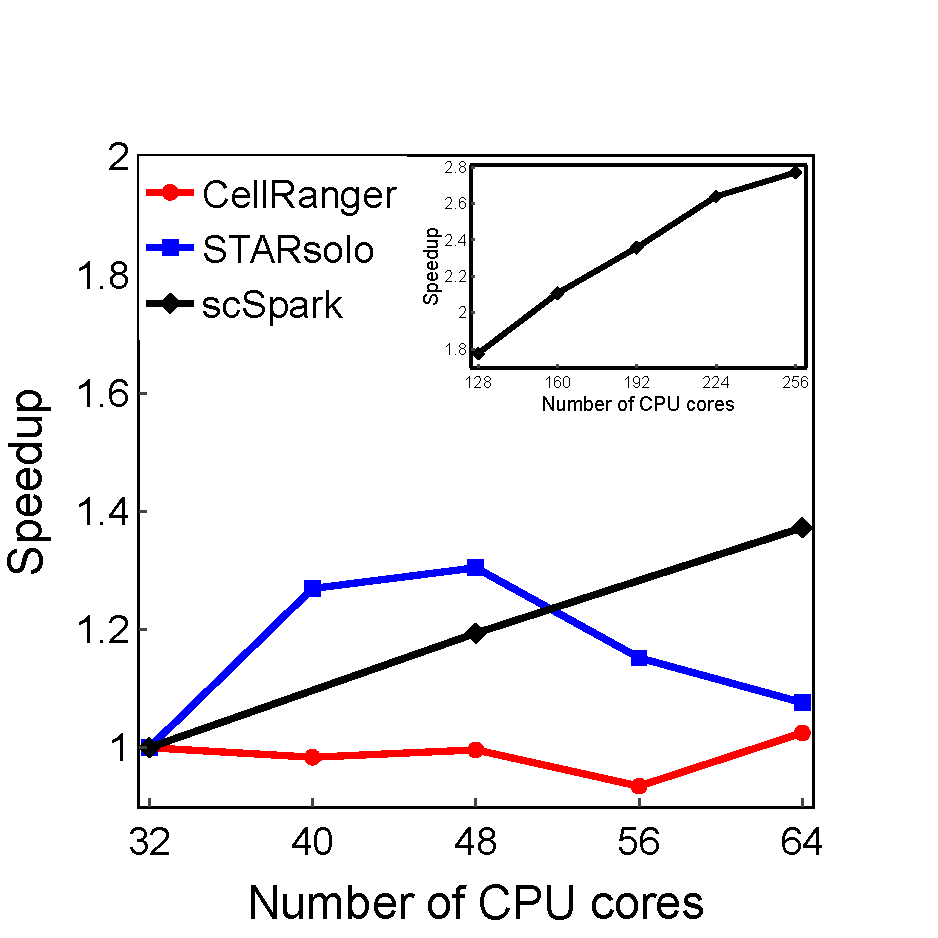
\includegraphics[width=0.72\textwidth]{fig3.pdf}
	\caption{scalability of each pipelines}
	\label{fig3}
\end{figure*}
\begin{figure*}
	\centering
	\subfigure[STAR's mapping speedup contrast with scSpark's mapping speed.]{\includegraphics[width=0.45\textwidth]{fig4a.pdf}}
	\subfigure[scSpark's mapping speed.]{\includegraphics[width=0.45\textwidth]{fig4b.pdf}}
	\caption{ pipelines' mapping speed. }
	\label{fig4}
\end{figure*}
\begin{figure}
	\centering
	\includegraphics[width=0.45\textwidth]{fig5.pdf}
	\caption{scSpark's speedup influenced by data volume.} \label{fig5}
\end{figure}

To identify whether scSpark get better performance than three state-of-the-art pipelines in same CPU cores number condition, we first evaluated the total time comsumption for different pipelines processing the same dataset with the same numbers of CPUs. 
For UMI-tools, CellRanger, and STARsolo, we used all 64 cores of a single workstation. 
For scSpark, we used a cluster of 4 computing nodes, where each node has 16 CPU cores. 
Results show that scSpark achieves substantially higher processing speed, which is nearly 20-fold faster than UMI-tools and about 5-fold faster than CellRanger and STARsolo (Table~\ref{tab1}). 

We also recorded the processing time for three individual modules of the pipelines, i.e., barcode extraction and sequence QC, genome alignment, and transcript quantification, to have a more detailed understanding of the performance gain. 
As scSpark is built based on UMI-tools, the breakdown comparison was only between UMI-tools and scSpark, to demonstrate the performance gain brought by distributed and in-memory computing.
Compared with UMI-tools, scSpark had significantly shorter processing time in all three steps (Fig.~\ref{fig2}).
It is noteworthy that scSpark achieved a processsing speed of approximately 50-fold faster than UMI-tools for the barcode extraction and sequence QC step, which turned out to be the dominant factor of the performance promotion brought by scSpark.
Moreover we found if scSpark and STAR both reduce genome load time that scSpark doesn't change STAR's tradition way, scSpark can get more than linear improve than STAR in align step which can prove scSpark can reduce align step's mapping time by reducing disk access.
The imporve in transcript counting step is influenced by data imbalance but its performance is more than 2-fold than UMI-tools.

This result reflects that distributed processing of FASTQ reads from disk and totally removal of re-writing temporary results back to disk that are both performed in scSpark can dramatically reduce the time consumption of scRNA-seq data processing pipelines. 

\subsection{Scalability evaluation}

\subsubsection{Scalability of each pipelines}
Contrast with traditional pipelines only can process on single workstation, scSpark can inherent process across Spark cluster.
So we think scSpark can inherent take advantange of scalability of Spark.
Therefore, to identified whether scSpark not only have more efficiency performance than traditional pipelines but also have more scalability with CPU cores number than traditional pipelines,
we computed the speedup of each tradition pipelines by considering 32 CPU cores execution times of each pipelines as a dividend and other numbers of CPU cores as divisor.
The scalability of pipeline is stronger if the speedup is bigger.

As Fig~\ref{fig3}.a shown, the speedup of STARsolo can get improve between 32 and 48 CPU cores.
Surprising, the performance of STARsolo in 48 CPU cores condition even more efficiency than the performance of STARsolo when CPU cores number bigger than 48.
This shows the scalability of STARsolo can get imporve when CPU cores number below a threshold but the improve of the performance of STARsolo can not scale-out with CPU cores number when CPU cores number bigger than the threshold.

As for CellRanger, we found when CPU cores number bigger than 32, the speedup of CellRanger can not take advantage of CPU cores number increase.
This shows CellRanger approximately lacks scalability when CPU cores number bigger than a threshold, in this case, the threshold is 32.

We found the speedup of scSpark is highest when CPU cores number is below 64.
Do not like the speedup of STARsolo and CellRanger, the speedup of scSpark is monotonically increasing with CPU cores number.
Furthermore, as Fig~\ref{fig3}.b shown, the speedup of scSpark achieve average 50\% improve when the CPU cores number of Spark cluster increased from 128 to 256.
This shows the scalability of scSpark not only have stable improve contrast with STARsolo and CellRanger, but also have more efficiency scalability than STARsolo and CellRanger.

In pretest, we found that the performance of UMI-tools can not take advantage of CPU core number increase because it only be supported on single\-thread mode except align step.
Although STAR can provides scalability on align step, the whole UMI-tools pipeline's scalability is weak.

So scSpark has most efficiency scalability in four pipelines when CPU cores number increase.

\subsubsection{Scalability of align step}
The aligner of all four pipelines is based on STAR, and in pretest shows the scalability of UMI-tools most comes from align step.
So we particulaly measured mapping speed of STAR and scSpark.

As Fig~\ref{fig4}.a shown, we found in align step, scSpark can get much higher mapping speed than STAR in any same CPU cores number condition.
This shows scSpark can take advantage of scSpark reimplement the method to storage the temporary result of pipeline in align step.
Furthermore, we found the mapping speed of scSpark can get nearly linear parallel efficiency with CPU cores number increase.
Although the mapping speed of STAR can get improve when CPU core number between 16 and 32, the improve of the mapping speed of STAR will converage when CPU cores number bigger than 32.
And as Fig~\ref{fig4}.b shown, the mapping speed of scSpark can get linear parallel efficiency even CPU cores number scale out to 256.
This shows the scalability of scSpark is much more efficiency than STAR in align step.

\subsubsection{The scalability of scSpark influenced of the volume of FASTQ data}
\begin{figure}
	\centering
	\includegraphics[width=0.45\textwidth]{fig6.pdf}
	\caption{correlation of scSpark and UMI-tools.} \label{fig6}
\end{figure}
\begin{figure*}
	\centering
	\includegraphics[width=0.9\textwidth]{fig7.pdf}
	\caption{tSNE picture based on scSpark and UMI-tools' gene expression matrix.} \label{fig7}
\end{figure*}
In experiment, we also found the performance of scSpark influenced by the volume of FASTQ data.
We think if the scalability of scSpark can improve with FASTQ

As Fig~\ref{fig5} shown, when FASTQ dataset contains 80 millions reads, the speedup of scSpark is much less than FASTQ dataset which contains 640 millions in CPU cores number between 128 and 256 condition.
Moreover, the speedup of scSpark will converage when dataset contains 80 millions reads or 160 millions reads and CPU cores number bigger than 192.
Contrast with small dataset, the speedup of scSpark can get increase when dataset contains 320 millions reads or 640 millions reads and CPU cores number bigger than 192.
So scSpark can scala-out more efficiency when scSpark processes larger dataset.

Our scSpark does not reimplement STAR's genome load method in align step which lack scalability in align step may be charged with some responsibility of scalability of scSpark scalability influenced by data volume.
We found both scSpark and STAR lack scalability in this substep because genome load method of STAR does not influencd by CPU cores number nor input dataset volume.
The process time of this substep occupy larger part of dataset which contains less reads causes the scalability of whole substep is weak. 

\subsection{Reliability of the results produced by scSpark} 
We further evaluated the accuracy of the expression matrices generated by scSpark.
First, the total UMI count for each cell in PBMC\_human dataset produced by scSpark was highly consistent with that by UMI-tools, with a Pearson correlation of $R^{2} = 0.9998$ (Fig~\ref{fig6}), which indicates that the expression profile of single cells produced by scSpark is reliable.
In addition, we also evaluated whether scSpark would have influence on downstream biological analysis.
Results show that the cell embeddings in tSNE map were highly consistent between scSpark and UMI-tools (Fig~\ref{fig7}).
This further demonstrates that the expression matrices generated by scSpark are accurate and would not bring interference to various types of downstream analysis such as clustering, dimension reduction and cell type identification.

\section{Conclusion}

In recent years, NGS methods proliferate the volume and value of scRNA-seq data, which requires more efficiency and scalability scRNASeq upstream pipelines.
Our scSpark is an efficiently, highly scalable and biological correct parallel compute scRNASeq upstream pipeline on the top of Spark.

In experiment, we believe our scSpark's strategy reduce the exection time with speedup between 5 and 20 times in 64 CPU cores condition.
And scSpark can scale-out more than 256 CPU cores contrast with tradition pipelines' performance will converage when workstation scale-out 64 CPU cores.
Moreover, we found scSpark shows more scalability when FASTQ dataset volume increase which means scSpark have potential to processed increasing FASTQ dataset by making Spark cluster bigger.
Importantly, we also believe that scSpark result biological was confirmed.

\bibliographystyle{IEEEtran}
\bibliography{reference}

\end{document}
